%%% - - -   UNCLASSIFIED   - - - %%%

%% ============================================================
%%  FRONT MATTER -- Title Page
%% ============================================================

\newcommand\VersionNumber{1.0}

\begin{center}
    \vspace*{0.3in}
    \Huge\textbf{\LARGE\unclass Interface Control Document\\}
    \vspace*{0.15in}
    \Large\textbf{\unclass T-150 UAS AFSIM Plugin Suite\\}
    \vspace*{0.3in}
    
\includegraphics[width=4in]{images/ngic}

    \vspace*{0.1in}
    \Large
    \textbf{Version: \VersionNumber \\
    Date: 5 March 2026 \\
    Classification: UNCLASSIFIED \\}
    \vspace*{0.1in}
    \normalsize
    \textbf{Prepared By: [PLACEHOLDER - Author Name]\\
    Organization: [PLACEHOLDER - Organization]\\
    Contract Number: [PLACEHOLDER]\\}
\end{center}

\vfill
\hfill
\begin{footnotesize}
    \begin{tabular}{|r@{: }l|}
    \hline
    Controlled by                        & [PLACEHOLDER]  \\
    Distribution/Dissemination Controls  & [PLACEHOLDER - Distribution Statement]  \\
    POC                                  & [PLACEHOLDER]  \\
    Contact                              & \ngicemail\\
    \hline
    \end{tabular}
\end{footnotesize}

\myemptypage

%% ============================================================
%%  Revision Table
%% ============================================================

\begin{center}
    \begin{tblr}
        {
            colspec     ={|Q[c,1in]|Q[c,1in]|Q[c,2in]|Q[2in]|},
            hline{1-Z}  ={.5pt},
            cell{1}{1}  ={c=4}{halign=l},
            cell{Z}{1}  ={c=4}{halign=r},
            row{2}      ={bg=TableBlue,fg=white,halign=c},
            cell{2-Y}{1}={halign=c},
        }
        \unclasslabel\\
        Revision & Date     & Author   & Description of Changes \\
        1.0     & 20260305 & {[PLACEHOLDER]}  & Initial release        \\
        \unclasslabel\\
    \end{tblr}
\end{center}

\vfill
\pagebreak

%% ============================================================
%%  TOC, LOT, LOF
%% ============================================================

\tableofcontents\thispagestyle{fancy}\pagebreak
\listoftables\thispagestyle{fancy}\pagebreak
\listoffigures\thispagestyle{fancy}\pagebreak

% arabic numbering and footer update
\pagenumbering{arabic}
\cfoot{\classlabel\ \\ {Page \thepage\ of \pageref{LastPage}}}


%% ============================================================
%%  SECTION 1 -- Introduction
%% ============================================================

\section{\unclass Introduction}

\subsection{\unclass Purpose}

\unclass This Interface Control Document (ICD) defines the software interfaces for the T-150 UAS AFSIM Plugin Suite. It specifies how each plugin communicates with the AFSIM simulation framework and with other plugins in the suite. The document serves as the authoritative reference for interface agreements between plugin components.

\unclass This document is adapted from the NGIC ICD template (originally designed for ODESSA DLL interfaces) to the AFSIM plugin architecture. The following mapping conventions apply:

\begin{itemize}
    \item \unclass ``DLL'' maps to ``Plugin (.dll/.so)''
    \item \unclass ``Structs'' maps to ``AuxData Key-Value Interface''
    \item \unclass ``DLL Functions'' maps to ``Plugin API Entry Points''
    \item \unclass Sections specific to RF, antenna patterns, or frequency interfaces are marked ``Not Applicable''
\end{itemize}

\subsection{\unclass Scope}

\unclass This ICD covers the five plugins comprising the T-150 UAS simulation capability:

\tableFivNow{\unclasslabel}{\unclass Plugin Suite Scope}{icd-scope}{l,1.5in}{l,1.5in}{l,1.3in}
{
    Plugin Library & Registered Type & Base Class \\
    t150\_battery (.dll/.so) & T150\_BATTERY\_PROCESSOR & WsfProcessor \\
    t150\_propulsion (.dll/.so) & T150\_PROPULSION\_PROCESSOR & WsfProcessor \\
    t150\_vrs (.dll/.so) & T150\_VRS\_PROCESSOR & WsfProcessor \\
    t150\_slung\_load (.dll/.so) & T150\_SLUNG\_LOAD\_PROCESSOR & WsfProcessor \\
    rotorcraft\_6dof (.dll/.so) & WSF\_ROTORCRAFT\_6DOF\_MOVER & WsfRouteMover \\
}

\unclass The document covers plugin loading, API entry points, inter-plugin data exchange via the AuxData key-value store, scenario configuration interfaces, and external output interfaces.

\subsection{\unclass Document Organization}

\begin{itemize}
    \item \unclass Section 2 describes how AFSIM discovers, loads, and initializes plugins.
    \item \unclass Section 3 specifies the required C-linkage entry points and registration classes.
    \item \unclass Section 4 defines the complete AuxData key-value interface organized by producer.
    \item \unclass Section 5 describes inter-plugin data flow and producer-consumer relationships.
    \item \unclass Section 6 documents the scenario script configuration interface.
    \item \unclass Section 7 covers external interfaces including file output and visualization.
    \item \unclass Sections 8 and 9 provide references and acronyms.
\end{itemize}

\subsection{\unclass Applicable Standards}

\begin{itemize}
    \item \unclass AFSIM Plugin API (version determined at compile time via \texttt{WSF\_PLUGIN\_API\_MAJOR\_VERSION} / \texttt{WSF\_PLUGIN\_API\_MINOR\_VERSION})
    \item \unclass C++17 language standard
    \item \unclass CMake 3.16+ build system
\end{itemize}

\pagebreak

%% ============================================================
%%  SECTION 2 -- Plugin Interface Overview
%% ============================================================

\section{\unclass Plugin Interface Overview}

\subsection{\unclass Plugin Discovery and Loading}

\unclass AFSIM discovers plugins by scanning shared library files in its plugin directories. On Linux, plugins are \texttt{.so} files; on Windows, \texttt{.dll} files. AFSIM loads each library and invokes standardized C-linkage entry points to negotiate version compatibility and register extensions.

\subsection{\unclass Plugin Directories}

\unclass Plugins must be installed to both AFSIM system directories to be discovered:

\tableTwoNow{\unclasslabel}{\unclass Plugin Directories}{icd-plugindirs}{l,2.5in}{l,3.5in}
{
    Directory & Purpose \\
    \texttt{<AFSIM\_ROOT>/lib/wsf\_plugins/} & Primary plugin search path \\
    \texttt{<AFSIM\_ROOT>/bin/mission\_plugins/} & Secondary plugin search path \\
}

\unclass On Linux, the typical AFSIM root is \texttt{/opt/afsim*/}. On Windows, it is the AFSIM installation directory. Plugins placed in project-local directories (e.g., \texttt{./lib/}) are \textbf{not} loaded by the AFSIM runtime.

\subsection{\unclass Plugin Lifecycle}

\unclass Each plugin follows a five-stage lifecycle:

\begin{figure}[H]
\begin{center}
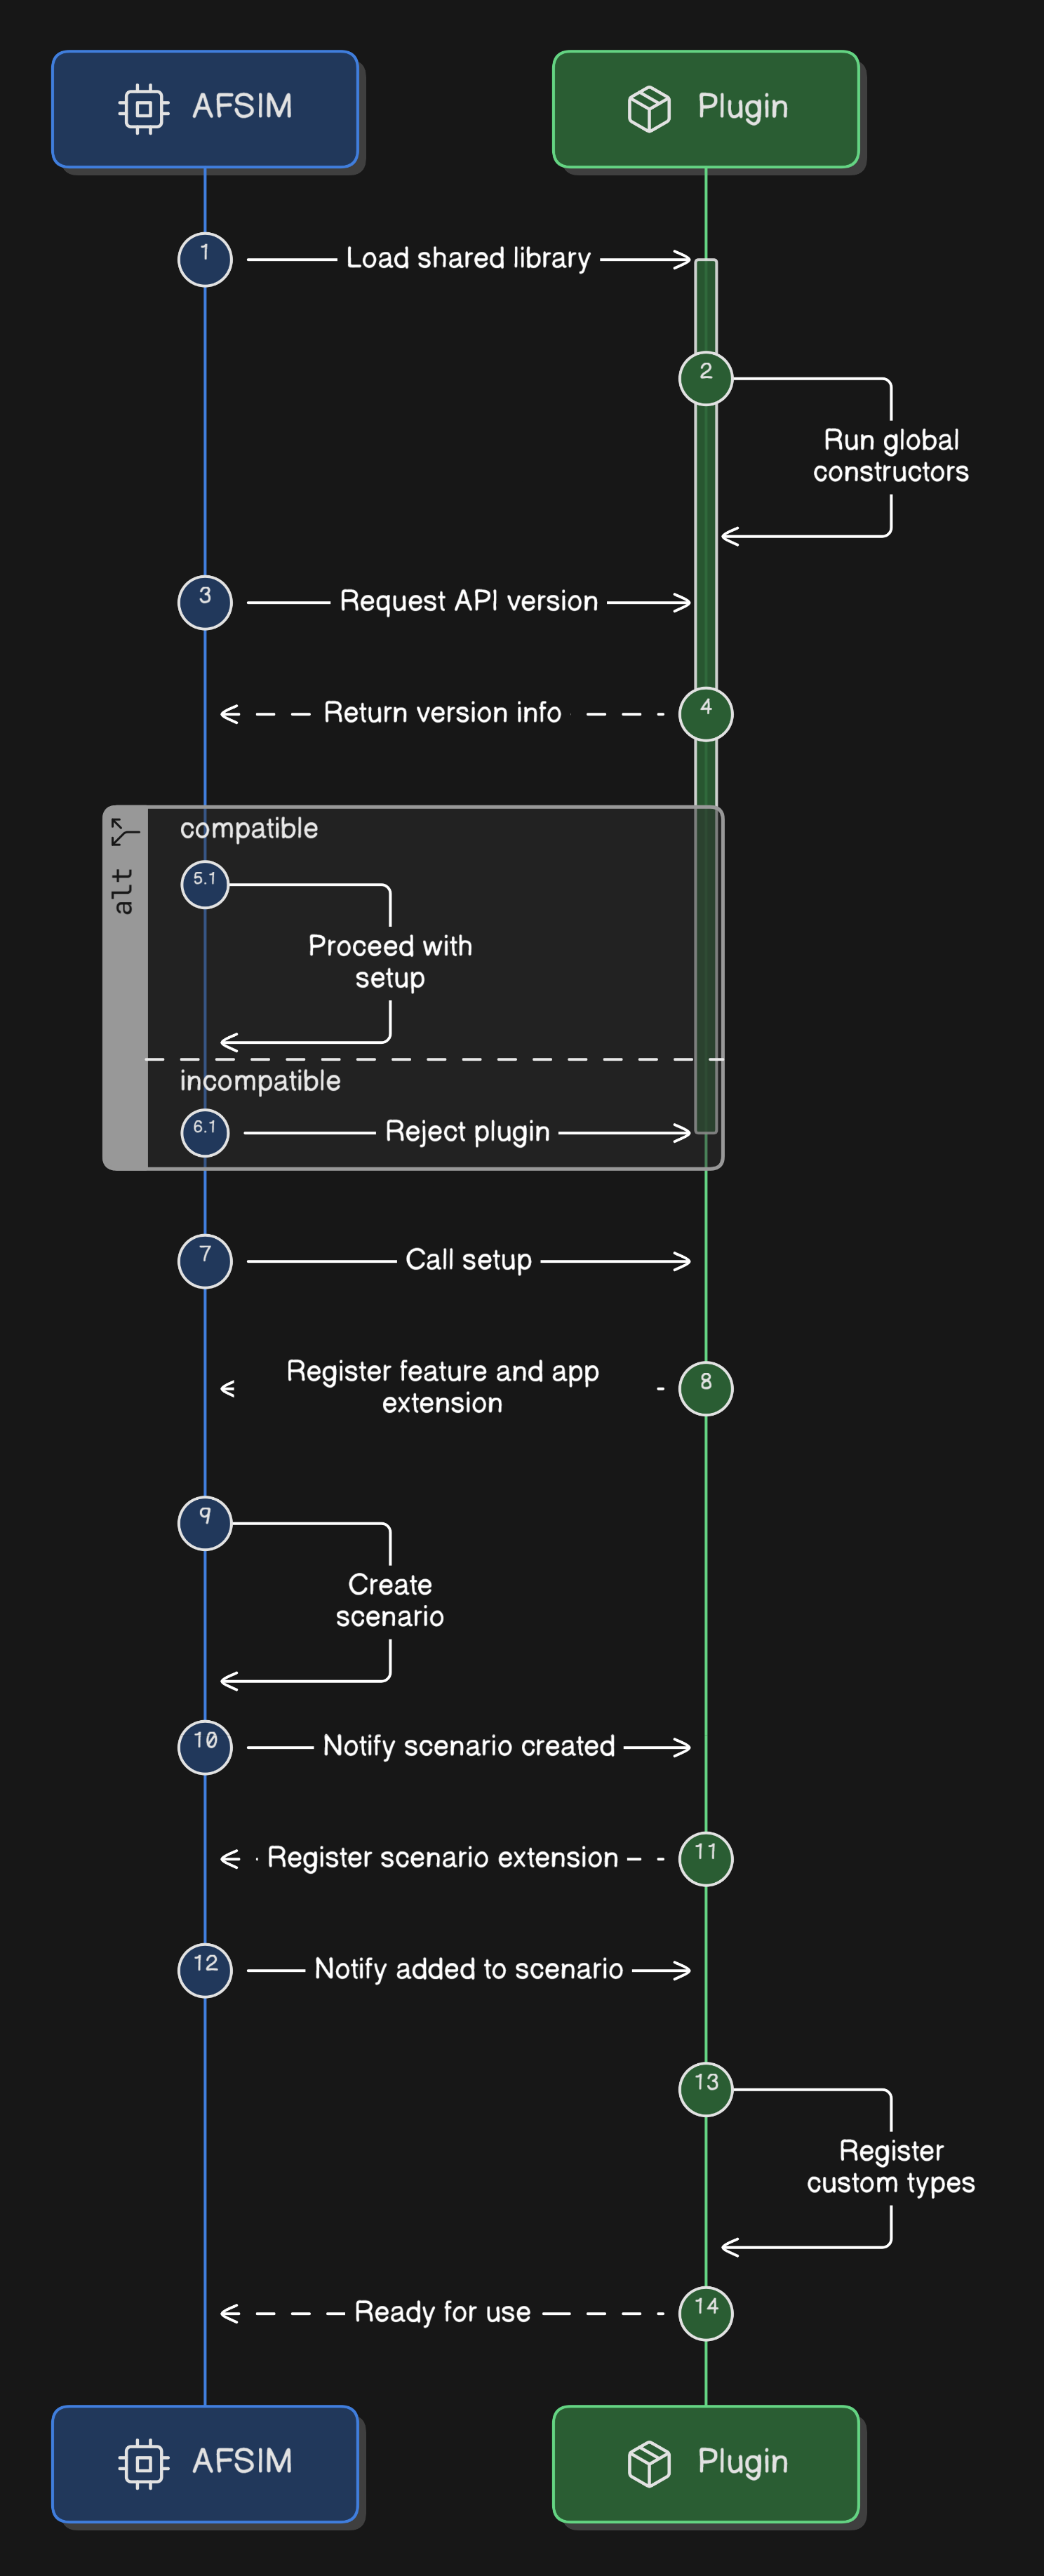
\includegraphics[width=0.9\textwidth,height=0.85\textheight,keepaspectratio]{images/16_ICD_plugin_lifecycle.png}
\caption{\unclass AFSIM Plugin Lifecycle}
\label{fig:pluginLifecycle}
\end{center}
\end{figure}

\subsection{\unclass Feature Registration}

\unclass Each plugin registers a feature name that scenario files can query to verify plugin availability:

\tableThrNow{\unclasslabel}{\unclass Feature Registration}{icd-features}{l,2in}{l,2in}{l,2in}
{
    Plugin & Feature Name & Extension Name \\
    t150\_battery & \texttt{t150\_battery} & \texttt{t150\_battery\_registration} \\
    t150\_propulsion & \texttt{t150\_propulsion} & \texttt{t150\_propulsion\_registration} \\
    t150\_vrs & \texttt{t150\_vrs} & \texttt{t150\_vrs\_registration} \\
    t150\_slung\_load & \texttt{t150\_slung\_load} & \texttt{t150\_slung\_load\_registration} \\
    rotorcraft\_6dof & \texttt{rotorcraft\_6dof} & \texttt{rotorcraft\_6dof\_registration} \\
}

\pagebreak

%% ============================================================
%%  SECTION 3 -- Plugin API Entry Points
%% ============================================================

\section{\unclass Plugin API Entry Points}

\subsection{\unclass Common Entry Points}

\unclass All five plugins export the same two C-linkage functions. The function signatures use AFSIM-provided types.

\subsubsection{\unclass WsfPluginVersion}

\begin{codebox}
\begin{lstlisting}[language=C++,mathescape=false]
extern "C" EXPORT_MACRO void WsfPluginVersion(UtPluginVersion& aVersion)
\end{lstlisting}
\end{codebox}

\unclass \textbf{Purpose:} Returns the AFSIM API version the plugin was compiled against.

\unclass \textbf{Behavior:} Constructs a \texttt{UtPluginVersion} from compile-time constants:

\tableTwoNow{\unclasslabel}{\unclass WsfPluginVersion Constants}{icd-versionconst}{l,2.5in}{l,3.5in}
{
    Constant & Description \\
    \texttt{WSF\_PLUGIN\_API\_MAJOR\_VERSION} & AFSIM major API version \\
    \texttt{WSF\_PLUGIN\_API\_MINOR\_VERSION} & AFSIM minor API version \\
    \texttt{WSF\_PLUGIN\_API\_SYSTEMABI\_STRING} & Platform ABI identifier \\
}

\unclass AFSIM compares these values against its own version. If the major version differs, the plugin is rejected.

\subsubsection{\unclass WsfPluginSetup}

\begin{codebox}
\begin{lstlisting}[language=C++,mathescape=false]
extern "C" EXPORT_MACRO void WsfPluginSetup(WsfApplication& aApplication)
\end{lstlisting}
\end{codebox}

\unclass \textbf{Purpose:} Registers the plugin's feature name and application extension.

\unclass \textbf{Behavior:}
\begin{enumerate}
    \item \unclass Checks \texttt{aApplication.ExtensionIsRegistered()} to prevent duplicate registration.
    \item \unclass Calls \texttt{aApplication.RegisterFeature()} with the plugin's feature name.
    \item \unclass Calls \texttt{aApplication.RegisterExtension()} with a new \texttt{ApplicationExtension} instance.
\end{enumerate}

\unclass The battery plugin additionally prints a CUI banner on first plugin load (coordinated via the \texttt{NGIC\_BANNER\_PRINTED} environment variable to print only once across all NGIC plugins).

\subsection{\unclass ApplicationExtension::ScenarioCreated}

\begin{codebox}
\begin{lstlisting}[language=C++,mathescape=false]
void ScenarioCreated(WsfScenario& aScenario) override
\end{lstlisting}
\end{codebox}

\unclass \textbf{Purpose:} Registers a \texttt{ScenarioExtension} with the newly created scenario.

\unclass \textbf{Behavior:} Calls \texttt{aScenario.RegisterExtension()} with a scenario-specific registration object. Most plugins use \texttt{WsfDefaultApplicationExtension<RegistrationType>} as a convenience wrapper. The battery plugin uses a custom \texttt{ApplicationExtension} class.

\subsection{\unclass ScenarioExtension::AddedToScenario}

\begin{codebox}
\begin{lstlisting}[language=C++,mathescape=false]
void AddedToScenario() override
\end{lstlisting}
\end{codebox}

\unclass \textbf{Purpose:} Registers the plugin's processor or mover type so that scenario files can instantiate it.

\unclass \textbf{Behavior by plugin:}

\tableThrNow{\unclasslabel}{\unclass Type Registration}{icd-typereg}{l,1.8in}{l,2.2in}{l,2in}
{
    Plugin & Registration Call & Type Name \\
    t150\_battery & \texttt{WsfProcessorTypes::Get(scen).AddCoreType(...)} & \texttt{T150\_BATTERY\_PROCESSOR} \\
    t150\_propulsion & \texttt{WsfProcessorTypes::Get(scen).AddCoreType(...)} & \texttt{T150\_PROPULSION\_PROCESSOR} \\
    t150\_vrs & \texttt{WsfProcessorTypes::Get(scen).AddCoreType(...)} & \texttt{T150\_VRS\_PROCESSOR} \\
    t150\_slung\_load & \texttt{WsfProcessorTypes::Get(scen).AddCoreType(...)} & \texttt{T150\_SLUNG\_LOAD\_PROCESSOR} \\
    rotorcraft\_6dof & \texttt{WsfMoverTypes::Get(scen).AddCoreType(...)} & \texttt{WSF\_ROTORCRAFT\_6DOF\_MOVER} \\
}

\unclass Each \texttt{AddCoreType} call provides a prototype instance that AFSIM clones (via the \texttt{Clone()} method) for each platform that uses that type.

\pagebreak

%% ============================================================
%%  SECTION 4 -- AuxData Interface
%% ============================================================

\section{\unclass AuxData Interface}

\unclass The AuxData interface is the primary mechanism for inter-plugin communication. Each plugin writes key-value pairs to the platform's \texttt{WsfAttributeContainer} (accessed via \texttt{GetPlatform()->GetAuxData()}). Other plugins and scenario scripts can read these values. All keys are string identifiers; values are typed as double, int, bool, or string.

\subsection{\unclass Battery Processor Outputs (9 Keys)}

\unclass Producer: \texttt{T150\_BATTERY\_PROCESSOR}

\tableFivNow{\unclasslabel}{\unclass Battery Processor AuxData Keys}{icd-batt-auxdata}{l,1.3in}{c,0.6in}{c,0.6in}{c,0.7in}{l,2.3in}
{
    AuxData Key & Type & Units & Range & Description \\
    \texttt{BATTERY\_SOC} & double & -- & 0.0--1.0 & State of charge (1.0 = fully charged) \\
    \texttt{BATTERY\_POWER\_W} & double & W & $\geq$ 0 & Current total electrical power draw \\
    \texttt{BATTERY\_ENERGY\_WH} & double & Wh & $\geq$ 0 & Remaining energy in battery \\
    \texttt{BATTERY\_VOLTAGE} & double & V & 39.0--54.6 & Terminal voltage under load \\
    \texttt{BATTERY\_OCV} & double & V & 39.0--54.6 & Open-circuit voltage (no-load) \\
    \texttt{BATTERY\_VOLTAGE\_SAG} & double & V & $\geq$ 0 & Voltage drop due to internal resistance \\
    \texttt{BATTERY\_CURRENT\_A} & double & A & $\geq$ 0 & Current draw from battery \\
    \texttt{BATTERY\_LOW} & bool & -- & true/false & SOC below low-battery threshold (default 20\%) \\
    \texttt{BATTERY\_VOLTAGE\_LOW} & bool & -- & true/false & Terminal voltage below sag warning level \\
}

\unclass \textbf{Update rate:} 10~Hz (100~ms update interval)

\unclass \textbf{Notes:} \texttt{BATTERY\_LOW} is set once when SOC drops below threshold and does not reset. \texttt{BATTERY\_VOLTAGE\_LOW} resets when voltage recovers above the warning level plus 1.0~V hysteresis.

\subsection{\unclass Propulsion Processor Outputs (19 Keys)}

\unclass Producer: \texttt{T150\_PROPULSION\_PROCESSOR}

\tableFivNow{\unclasslabel}{\unclass Propulsion Processor AuxData Keys}{icd-prop-auxdata}{l,1.3in}{c,0.6in}{c,0.6in}{c,0.7in}{l,2.3in}
{
    AuxData Key & Type & Units & Range & Description \\
    \texttt{PROP\_TOTAL\_THRUST} & double & N & $\geq$ 0 & Total thrust from all rotors (with ground effect) \\
    \texttt{PROP\_TOTAL\_POWER} & double & W & $\geq$ 0 & Total electrical power consumption \\
    \texttt{PROP\_SYSTEM\_EFF} & double & -- & 0.0--1.0 & Overall system efficiency (motor $\times$ coaxial) \\
    \texttt{PROP\_MOTOR\_COUNT} & int & count & 0--8 & Number of currently operational motors \\
    \texttt{PROP\_MAX\_TEMP} & double & $^\circ$C & -40--200 & Hottest motor temperature \\
    \texttt{PROP\_AVG\_TEMP} & double & $^\circ$C & -40--200 & Average motor temperature \\
    \texttt{PROP\_GROUND\_EFFECT} & double & -- & 1.0--1.3 & Ground effect thrust multiplier \\
    \texttt{PROP\_ALTITUDE\_AGL} & double & m & $\geq$ 0 & Current altitude above ground level \\
    \texttt{PROP\_TOTAL\_MASS} & double & kg & $>$ 0 & Total mass (empty + payload) \\
    \texttt{PROP\_PAYLOAD\_MASS} & double & kg & $\geq$ 0 & Payload mass \\
    \texttt{PROP\_THRUST\_MARGIN} & double & -- & 0.0--1.0 & Available thrust margin above hover \\
    \texttt{PROP\_CG\_OFFSET\_X} & double & m & any & Combined CG offset, forward axis \\
    \texttt{PROP\_CG\_OFFSET\_Y} & double & m & any & Combined CG offset, lateral axis \\
    \texttt{PROP\_CG\_OFFSET\_Z} & double & m & any & Combined CG offset, vertical axis \\
    \texttt{PROP\_OVERLOADED} & bool & -- & true/false & Payload exceeds max capacity \\
    \texttt{PROP\_FORWARD\_SPEED} & double & m/s & $\geq$ 0 & Horizontal ground speed \\
    \texttt{PROP\_CLIMB\_RATE} & double & m/s & any & Vertical speed (positive = climbing) \\
    \texttt{PROP\_BANK\_ANGLE} & double & deg & 0--60 & Estimated bank angle \\
    \texttt{PROP\_ACCEL\_MAG} & double & m/s$^2$ & $\geq$ 0 & Horizontal acceleration magnitude \\
}

\unclass \textbf{Update rate:} 10~Hz (100~ms update interval)

\subsection{\unclass VRS Processor Outputs (10 Keys)}

\unclass Producer: \texttt{T150\_VRS\_PROCESSOR}

\tableFivNow{\unclasslabel}{\unclass VRS Processor AuxData Keys}{icd-vrs-auxdata}{l,1.3in}{c,0.6in}{c,0.6in}{c,0.7in}{l,2.3in}
{
    AuxData Key & Type & Units & Range & Description \\
    \texttt{VRS\_MARGIN} & double & -- & 0.0--1.0 & Distance from VRS boundary (0 = in VRS, 1 = clear) \\
    \texttt{VRS\_STATE} & int & enum & 0--4 & VRS state machine value (see below) \\
    \texttt{VRS\_LIFT\_FACTOR} & double & -- & 0.4--1.0 & Lift degradation factor (1.0 = no degradation) \\
    \texttt{VRS\_CONTROL\_FACTOR} & double & -- & 0.5--1.0 & Control authority factor (1.0 = full authority) \\
    \texttt{VRS\_DEVELOPMENT} & double & -- & 0.0--1.0 & VRS development progression \\
    \texttt{VRS\_DESCENT\_RATE} & double & m/s & $\geq$ 0 & Current descent rate (positive = descending) \\
    \texttt{VRS\_FORWARD\_SPEED} & double & m/s & $\geq$ 0 & Current horizontal speed \\
    \texttt{VRS\_CAUTION} & bool & -- & true/false & Approaching VRS envelope \\
    \texttt{VRS\_ONSET} & bool & -- & true/false & VRS onset detected \\
    \texttt{VRS\_CRITICAL} & bool & -- & true/false & VRS fully developed, recovery action required \\
}

\unclass \textbf{VRS\_STATE enum values:}

\tableTwoNow{\unclasslabel}{\unclass VRS State Enumeration}{icd-vrs-states}{c,0.5in}{l,5in}
{
    Value & Description \\
    0 & CLEAR -- No VRS risk \\
    1 & CAUTION -- Approaching VRS boundary \\
    2 & ONSET -- VRS conditions beginning \\
    3 & DEVELOPED -- Full VRS, severe lift/control degradation \\
    4 & RECOVERY -- Transitioning out of VRS \\
}

\unclass \textbf{Update rate:} 10~Hz (100~ms update interval)

\subsection{\unclass Slung Load Processor Outputs (14 Keys)}

\unclass Producer: \texttt{T150\_SLUNG\_LOAD\_PROCESSOR}

\tableFivNow{\unclasslabel}{\unclass Slung Load Processor AuxData Keys}{icd-slung-auxdata}{l,1.3in}{c,0.6in}{c,0.6in}{c,0.7in}{l,2.3in}
{
    AuxData Key & Type & Units & Range & Description \\
    \texttt{SLUNG\_LOAD\_STATE} & int & enum & 0--4 & Load state (see below) \\
    \texttt{SLUNG\_LOAD\_MASS} & double & kg & $\geq$ 0 & Attached load mass \\
    \texttt{SLUNG\_CABLE\_LENGTH} & double & m & $\geq$ 0.5 & Cable length \\
    \texttt{SLUNG\_CABLE\_TENSION} & double & N & $\geq$ 0 & Current cable tension \\
    \texttt{SLUNG\_SWING\_X} & double & deg & -70--70 & Pendulum angle in pitch (X-Z plane) \\
    \texttt{SLUNG\_SWING\_Y} & double & deg & -70--70 & Pendulum angle in roll (Y-Z plane) \\
    \texttt{SLUNG\_SWING\_MAG} & double & deg & 0--70 & Combined swing angle magnitude \\
    \texttt{SLUNG\_FORCE\_X} & double & N & any & Cable reaction force on aircraft, forward axis \\
    \texttt{SLUNG\_FORCE\_Y} & double & N & any & Cable reaction force on aircraft, lateral axis \\
    \texttt{SLUNG\_FORCE\_Z} & double & N & $\geq$ 0 & Cable reaction force on aircraft, vertical axis \\
    \texttt{SLUNG\_POS\_X} & double & m & any & Load position relative to aircraft CG, forward \\
    \texttt{SLUNG\_POS\_Y} & double & m & any & Load position relative to aircraft CG, lateral \\
    \texttt{SLUNG\_POS\_Z} & double & m & any & Load position relative to aircraft CG, vertical \\
    \texttt{SLUNG\_NATURAL\_FREQ} & double & Hz & $>$ 0 & Pendulum natural frequency \\
    \texttt{SLUNG\_RESONANCE} & bool & -- & true/false & Resonance condition detected \\
}

\unclass \textbf{SLUNG\_LOAD\_STATE enum values:}

\tableTwoNow{\unclasslabel}{\unclass Slung Load State Enumeration}{icd-slung-states}{c,0.5in}{l,5in}
{
    Value & Description \\
    0 & DETACHED -- No load attached \\
    1 & ATTACHED -- Load attached, stable \\
    2 & SWINGING -- Swing exceeds resonance threshold \\
    3 & RESONANCE -- Swing frequency matches natural frequency at large amplitude \\
    4 & RELEASED -- Load released (cable overload or commanded) \\
}

\unclass \textbf{Update rate:} 50~Hz (20~ms update interval, configurable)

\subsection{\unclass 6DOF Mover Outputs (16 Keys)}

\unclass Producer: \texttt{WSF\_ROTORCRAFT\_6DOF\_MOVER}

\tableFouNow{\unclasslabel}{\unclass 6DOF Mover AuxData Keys}{icd-6dof-auxdata}{l,1.3in}{c,0.6in}{c,0.6in}{l,3in}
{
    AuxData Key & Type & Units & Description \\
    \texttt{6dof\_pos\_n} & double & m & Local NED position, North \\
    \texttt{6dof\_pos\_e} & double & m & Local NED position, East \\
    \texttt{6dof\_pos\_d} & double & m & Local NED position, Down \\
    \texttt{6dof\_vel\_n} & double & m/s & NED velocity, North \\
    \texttt{6dof\_vel\_e} & double & m/s & NED velocity, East \\
    \texttt{6dof\_vel\_d} & double & m/s & NED velocity, Down (positive = descending) \\
    \texttt{6dof\_roll\_deg} & double & deg & Roll angle \\
    \texttt{6dof\_pitch\_deg} & double & deg & Pitch angle \\
    \texttt{6dof\_yaw\_deg} & double & deg & Yaw angle (heading) \\
    \texttt{6dof\_p\_dps} & double & deg/s & Roll rate \\
    \texttt{6dof\_q\_dps} & double & deg/s & Pitch rate \\
    \texttt{6dof\_r\_dps} & double & deg/s & Yaw rate \\
    \texttt{6dof\_total\_thrust} & double & N & Total rotor thrust \\
    \texttt{6dof\_total\_power} & double & W & Total mechanical power (shaft) \\
    \texttt{6dof\_throttle\_cmd} & double & 0--1 & Throttle command \\
    \texttt{6dof\_avg\_rpm} & double & RPM & Average rotor RPM \\
    \texttt{6dof\_mass} & double & kg & Current aircraft mass \\
    \texttt{6dof\_weight} & double & N & Current weight force \\
    \texttt{6dof\_target\_alt} & double & m MSL & Target altitude \\
}

\unclass \textbf{Update rate:} 100~Hz (10~ms update interval)

\subsection{\unclass 6DOF Mover Consumed Keys}

\unclass The 6DOF mover reads AuxData keys published by other processors to integrate external forces and moments:

\tableThrNow{\unclasslabel}{\unclass 6DOF Mover Consumed AuxData Keys}{icd-6dof-consumed}{l,2in}{l,1.5in}{l,2.5in}
{
    Consumed Key & Source Plugin & Purpose \\
    \texttt{SLUNG\_FORCE\_X/Y/Z} & Slung Load Processor & Cable reaction forces on aircraft \\
    \texttt{WEAPON\_FORCE\_X/Y/Z} & Weapon Processor (legacy) & Weapon recoil forces \\
    \texttt{WEAPON\_<name>\_FORCE\_X/Y/Z} & Weapon Processor (registry) & Per-weapon recoil forces \\
    \texttt{WEAPON\_MOMENT\_X/Y/Z} & Weapon Processor (legacy) & Weapon recoil moments \\
    \texttt{WEAPON\_<name>\_MOMENT\_X/Y/Z} & Weapon Processor (registry) & Per-weapon recoil moments \\
    \texttt{WEAPON\_REGISTRY} & Weapon Processor & Comma-separated list of weapon names \\
    \texttt{WEAPON\_<name>\_MASS\_DELTA} & Weapon Processor & Ammunition mass change per weapon \\
}

\pagebreak

%% ============================================================
%%  SECTION 5 -- Inter-Plugin Data Flow
%% ============================================================

\section{\unclass Inter-Plugin Data Flow}

\subsection{\unclass Data Flow Diagram}

\begin{figure}[H]
\begin{center}
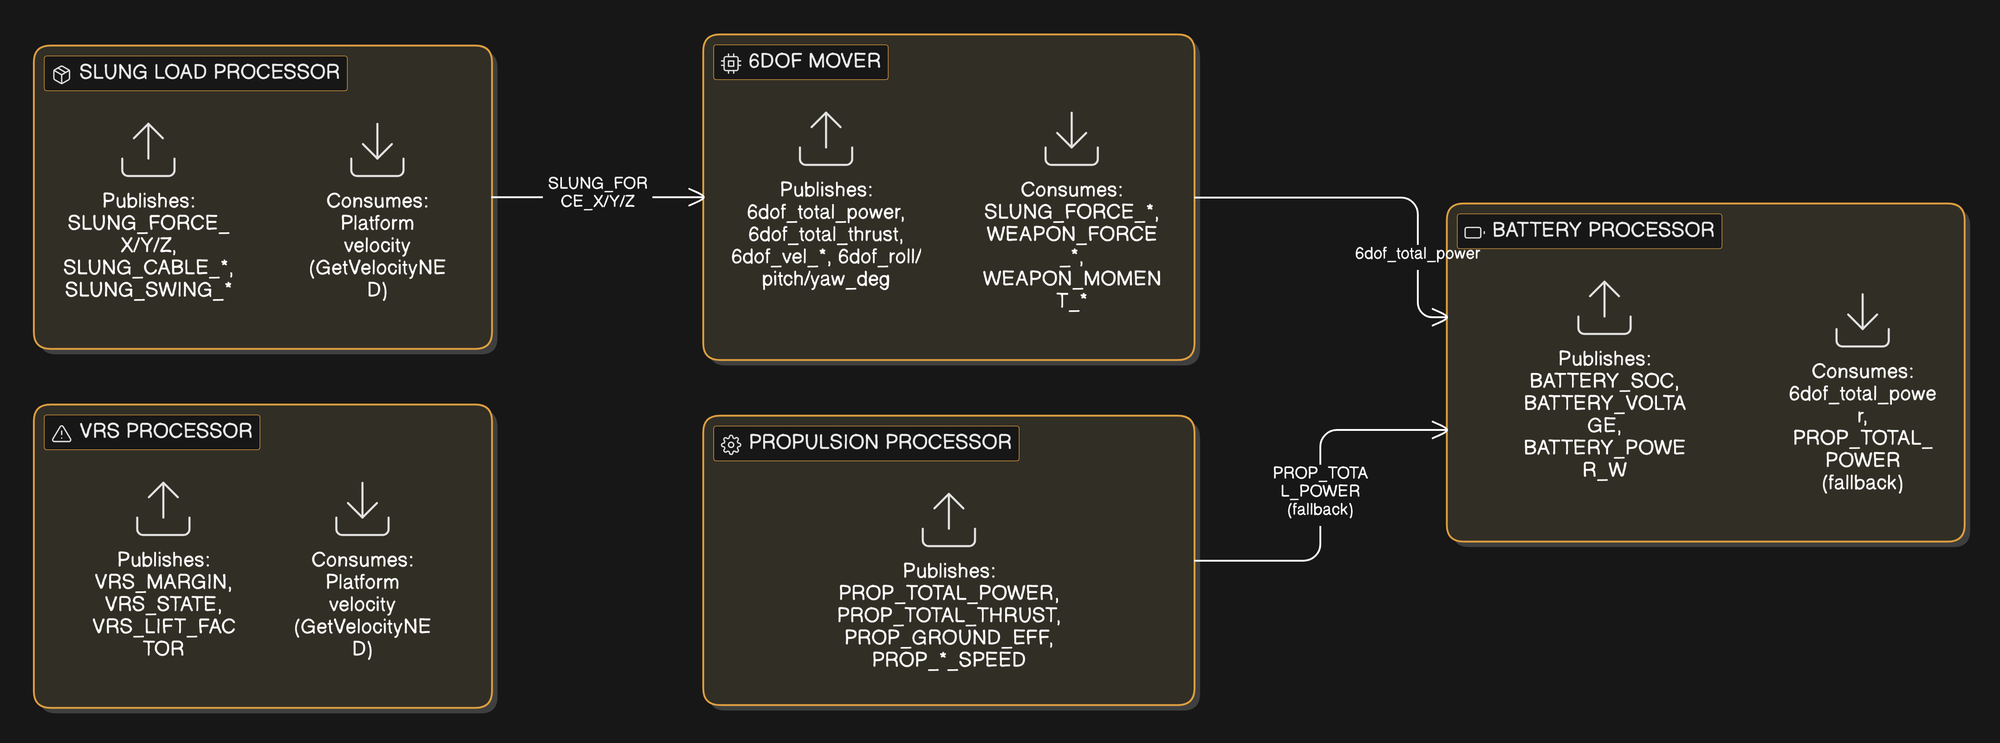
\includegraphics[width=\textwidth,height=0.85\textheight,keepaspectratio]{images/17_ICD_inter_plugin_data_flow.png}
\caption{\unclass Inter-Plugin Data Flow}
\label{fig:interPluginDataFlow}
\end{center}
\end{figure}

\subsection{\unclass Producer-Consumer Relationships}

\tableFivNow{\unclasslabel}{\unclass Producer-Consumer Data Paths}{icd-dataflow}{l,1.3in}{l,1.1in}{l,1.1in}{l,1.1in}{l,1in}
{
    Data Path & Producer & Consumer & Key(s) & Direction \\
    Mover power to battery & 6DOF Mover & Battery Proc. & \texttt{6dof\_total\_power} & Mover $\rightarrow$ Battery \\
    Propulsion power to battery & Propulsion Proc. & Battery Proc. & \texttt{PROP\_TOTAL\_POWER} & Prop $\rightarrow$ Battery (fallback) \\
    Slung load forces to mover & Slung Load Proc. & 6DOF Mover & \texttt{SLUNG\_FORCE\_X/Y/Z} & Slung Load $\rightarrow$ Mover \\
    Platform velocity to VRS & AFSIM Mover & VRS Proc. & \texttt{GetVelocityNED()} & Platform API \\
    Platform velocity to slung load & AFSIM Mover & Slung Load Proc. & \texttt{GetVelocityNED()} & Platform API \\
}

\subsection{\unclass Battery Power Source Fallback Chain}

\unclass The Battery Processor uses a three-level fallback chain when \texttt{use\_dynamic\_power} is enabled:

\begin{enumerate}
    \item \unclass \textbf{Configured key} -- reads from \texttt{power\_source\_key} (default: \texttt{PROP\_TOTAL\_POWER}, typically overridden to \texttt{6dof\_total\_power})
    \item \unclass \textbf{6DOF mover power} -- reads \texttt{6dof\_total\_power} if the configured key returns zero or is absent
    \item \unclass \textbf{Propulsion processor power} -- reads \texttt{PROP\_TOTAL\_POWER} if neither of the above yields a positive value
    \item \unclass \textbf{Fixed fallback} -- uses \texttt{hover\_power\_w} if no dynamic source is available
\end{enumerate}

\subsection{\unclass Platform API Interfaces}

\unclass The VRS Processor and Slung Load Processor do not consume AuxData from other plugins. Instead, they read flight state directly from the AFSIM platform API:

\begin{itemize}
    \item \unclass \texttt{GetPlatform()->GetVelocityNED(velocityNED)} -- provides NED velocity vector
    \item \unclass \texttt{GetPlatform()->GetAltitude()} -- provides altitude MSL
\end{itemize}

\unclass Both processors derive acceleration by numerical differentiation of velocity across timesteps, with acceleration values clamped to filter numerical noise.

\pagebreak

%% ============================================================
%%  SECTION 6 -- Scenario Script Interface
%% ============================================================

\section{\unclass Scenario Script Interface}

\subsection{\unclass Configuration Mechanism}

\unclass Each plugin parses its configuration via the \texttt{ProcessInput(UtInput\& aInput)} method. AFSIM calls this method for each line within a \texttt{processor ... end\_processor} or \texttt{mover ... end\_mover} block in the scenario file. The method reads the command keyword via \texttt{aInput.GetCommand()} and the value via \texttt{aInput.ReadValue()} or \texttt{aInput.ReadBool()}.

\subsection{\unclass String Parameter Quote Stripping}

\unclass AFSIM's \texttt{ReadValue()} for string parameters includes surrounding double quotes in the returned value. Plugins that accept string parameters (e.g., \texttt{power\_source\_key}, \texttt{csv\_output\_file}) must strip these quotes. The Battery Processor implements this explicitly:

\begin{codebox}
\begin{lstlisting}[language=C++,mathescape=false]
if (mPowerSourceKey.front() == '"' && mPowerSourceKey.back() == '"')
    mPowerSourceKey = mPowerSourceKey.substr(1, mPowerSourceKey.size() - 2);
\end{lstlisting}
\end{codebox}

\unclass Scenario authors must enclose string values in quotes: \texttt{power\_source\_key "6dof\_total\_power"}.

\subsection{\unclass Battery Processor Configuration Parameters}

\unclass Type name: \texttt{T150\_BATTERY\_PROCESSOR}

\tableFivNow{\unclasslabel}{\unclass Battery Processor Configuration}{icd-batt-config}{l,1.5in}{c,0.5in}{c,0.6in}{c,0.5in}{l,2.5in}
{
    Parameter & Type & Default & Units & Description \\
    \texttt{battery\_capacity\_wh} & double & 7000.0 & Wh & Total battery energy capacity \\
    \texttt{initial\_soc} & double & 1.0 & 0--1 & Starting state of charge \\
    \texttt{hover\_power\_w} & double & 18000.0 & W & Fallback hover power consumption \\
    \texttt{low\_battery\_warning} & double & 0.20 & 0--1 & SOC threshold for low battery warning \\
    \texttt{nominal\_voltage} & double & 46.8 & V & Nominal pack voltage \\
    \texttt{full\_charge\_voltage} & double & 54.6 & V & Full charge pack voltage \\
    \texttt{cutoff\_voltage} & double & 39.0 & V & Discharge cutoff voltage \\
    \texttt{internal\_resistance} & double & 0.025 & $\Omega$ & Pack internal resistance \\
    \texttt{voltage\_sag\_warning} & double & 42.0 & V & Voltage warning threshold \\
    \texttt{use\_dynamic\_power} & bool & false & -- & Enable reading power from AuxData \\
    \texttt{power\_source\_key} & string & PROP\_ TOTAL\_ POWER & -- & AuxData key for power input \\
    \texttt{auxiliary\_power\_w} & double & 4000.0 & W & Constant auxiliary systems draw \\
    \texttt{motor\_efficiency} & double & 0.85 & 0.1--1.0 & Mechanical-to-electrical conversion \\
    \texttt{min\_flight\_power\_factor} & double & 0.50 & 0.1--1.0 & Min power as fraction of hover \\
    \texttt{cruise\_power\_w} & double & 17000.0 & W & Power at cruise speed \\
    \texttt{cruise\_speed\_mps} & double & 30.0 & m/s & Cruise speed for velocity model \\
    \texttt{use\_velocity\_power\_model} & bool & true & -- & Enable velocity-based power estimation \\
    \texttt{csv\_output\_file} & string & (empty) & path & CSV telemetry output file path \\
    \texttt{csv\_log\_interval} & double & 1.0 & s & Interval between CSV log entries \\
}

\unclass \textbf{Example scenario configuration:}

\begin{codebox}
\begin{lstlisting}[language={},mathescape=false]
processor battery_monitor T150_BATTERY_PROCESSOR
   battery_capacity_wh 7000
   initial_soc 1.0
   nominal_voltage 46.8
   full_charge_voltage 54.6
   cutoff_voltage 39.0
   internal_resistance 0.025
   use_dynamic_power true
   power_source_key "6dof_total_power"
   hover_power_w 18000
   motor_efficiency 0.37
   auxiliary_power_w 4000
   use_velocity_power_model false
   csv_output_file /path/to/output/battery.csv
   csv_log_interval 1.0
end_processor
\end{lstlisting}
\end{codebox}

\subsection{\unclass Propulsion Processor Configuration Parameters}

\unclass Type name: \texttt{T150\_PROPULSION\_PROCESSOR}

\tableFivNow{\unclasslabel}{\unclass Propulsion Processor Configuration}{icd-prop-config}{l,1.5in}{c,0.5in}{c,0.6in}{c,0.5in}{l,2.5in}
{
    Parameter & Type & Default & Units & Description \\
    \texttt{motor\_count} & int & 8 & count & Number of motors (max 8) \\
    \texttt{kv\_rating} & double & 100.0 & RPM/V & Motor Kv rating \\
    \texttt{max\_power\_per\_motor} & double & 3500.0 & W & Maximum power per motor \\
    \texttt{propeller\_diameter} & double & 0.76 & m & Propeller diameter \\
    \texttt{coaxial\_efficiency} & double & 0.85 & 0.5--1.0 & Coaxial rotor interference factor \\
    \texttt{motor\_thermal\_limit} & double & 120.0 & $^\circ$C & Motor overtemperature threshold \\
    \texttt{esc\_thermal\_limit} & double & 90.0 & $^\circ$C & ESC overtemperature threshold \\
    \texttt{nominal\_voltage} & double & 46.8 & V & Battery pack nominal voltage \\
    \texttt{peak\_motor\_efficiency} & double & 0.92 & 0.5--0.98 & Peak motor efficiency \\
    \texttt{ambient\_temperature} & double & 25.0 & $^\circ$C & Ambient temperature \\
    \texttt{motor\_time\_constant} & double & 0.15 & s & First-order motor lag time constant \\
    \texttt{ground\_effect\_enabled} & bool & true & -- & Enable ground effect model \\
    \texttt{rotor\_height} & double & 0.5 & m & Rotor height above ground reference \\
    \texttt{ground\_effect\_max\_boost} & double & 1.3 & 1.0--1.5 & Max ground effect thrust multiplier \\
    \texttt{empty\_mass} & double & 68.0 & kg & Aircraft empty mass \\
    \texttt{payload\_mass} & double & 0.0 & kg & Payload mass \\
    \texttt{max\_payload\_mass} & double & 55.0 & kg & Maximum payload capacity \\
    \texttt{payload\_cg\_offset\_x/y/z} & double & 0/0/0.2 & m & Payload CG offset from aircraft CG \\
    \texttt{drag\_coefficient} & double & 1.0 & 0.1--2.0 & Bluff body drag coefficient \\
    \texttt{frontal\_area} & double & 0.30 & m$^2$ & Frontal reference area \\
    \texttt{induced\_power\_factor} & double & 1.15 & 1.0--1.5 & Non-ideal rotor power factor \\
    \texttt{csv\_output\_file} & string & (empty) & path & CSV telemetry output file path \\
    \texttt{csv\_log\_interval} & double & 1.0 & s & Interval between CSV log entries \\
}

\subsection{\unclass VRS Processor Configuration Parameters}

\unclass Type name: \texttt{T150\_VRS\_PROCESSOR}

\tableFivNow{\unclasslabel}{\unclass VRS Processor Configuration}{icd-vrs-config}{l,1.5in}{c,0.5in}{c,0.6in}{c,0.5in}{l,2.5in}
{
    Parameter & Type & Default & Units & Description \\
    \texttt{vrs\_descent\_threshold} & double & 4.0 & m/s & Descent rate for VRS onset \\
    \texttt{vrs\_speed\_threshold} & double & 5.0 & m/s & Forward speed that prevents VRS \\
    \texttt{caution\_margin} & double & 0.8 & 0.5--0.95 & VRS margin level for caution \\
    \texttt{induced\_velocity} & double & 8.0 & m/s & Estimated hover induced velocity \\
    \texttt{coaxial\_factor} & double & 0.85 & 0.5--1.0 & Coaxial rotor VRS resistance factor \\
    \texttt{vrs\_development\_time} & double & 2.0 & s & Time to develop full VRS \\
    \texttt{vrs\_recovery\_time} & double & 3.0 & s & Time to recover from VRS \\
    \texttt{max\_lift\_degradation} & double & 0.6 & 0.0--1.0 & Maximum lift loss fraction in VRS \\
    \texttt{max\_control\_degradation} & double & 0.5 & 0.0--1.0 & Maximum control authority loss in VRS \\
}

\subsection{\unclass Slung Load Processor Configuration Parameters}

\unclass Type name: \texttt{T150\_SLUNG\_LOAD\_PROCESSOR}

\tableFivNow{\unclasslabel}{\unclass Slung Load Processor Configuration}{icd-slung-config}{l,1.5in}{c,0.5in}{c,0.6in}{c,0.5in}{l,2.5in}
{
    Parameter & Type & Default & Units & Description \\
    \texttt{load\_mass} & double & 0.0 & kg & Attached load mass ($>$0 auto-attaches) \\
    \texttt{cable\_length} & double & 5.0 & m & Cable length (min 0.5~m) \\
    \texttt{cable\_damping} & double & 0.1 & -- & Pendulum damping coefficient \\
    \texttt{attach\_point\_x/y/z} & double & 0/0/0.5 & m & Cable attach point relative to CG \\
    \texttt{max\_cable\_tension} & double & 5000.0 & N & Cable tension limit (triggers release) \\
    \texttt{resonance\_threshold} & double & 20.0 & deg & Swing angle for resonance warning \\
    \texttt{update\_interval} & double & 0.02 & s & Physics update interval (min 1~ms) \\
}

\subsection{\unclass 6DOF Mover Configuration Parameters}

\unclass Type name: \texttt{WSF\_ROTORCRAFT\_6DOF\_MOVER}

\unclass The 6DOF mover inherits route-handling parameters from \texttt{WsfRouteMover} and adds physics configuration:

\tableFivNow{\unclasslabel}{\unclass 6DOF Mover Configuration}{icd-6dof-config}{l,1.5in}{c,0.5in}{c,0.6in}{c,0.5in}{l,2.5in}
{
    Parameter & Type & Default & Units & Description \\
    \texttt{mass} & double & -- & kg & Total aircraft mass \\
    \texttt{inertia\_xx/yy/zz} & double & -- & kg$\cdot$m$^2$ & Moments of inertia \\
    \texttt{rotor\_configuration} & string & -- & -- & COAXIAL\_QUAD, COAXIAL\_HEX, etc. \\
    \texttt{rotor\_diameter} & double & -- & m & Rotor/propeller diameter \\
    \texttt{arm\_length} & double & -- & m & Motor arm length from CG \\
    \texttt{coaxial\_spacing} & double & -- & m & Vertical spacing between coaxial rotors \\
    \texttt{thrust\_coefficient} & double & -- & -- & Rotor thrust coefficient (Ct) \\
    \texttt{torque\_coefficient} & double & -- & -- & Rotor torque coefficient (Cq) \\
    \texttt{max\_rpm} & double & -- & RPM & Maximum rotor RPM \\
    \texttt{motor\_time\_constant} & double & -- & s & Motor first-order lag \\
    \texttt{drag\_enabled} & bool & -- & -- & Enable aerodynamic drag model \\
    \texttt{drag\_coefficient\_x/y/z} & double & -- & -- & Directional drag coefficients \\
    \texttt{frontal\_area} & double & -- & m$^2$ & Reference frontal area \\
    \texttt{ground\_effect\_enabled} & bool & -- & -- & Enable ground effect model \\
    \texttt{ground\_effect\_height\_factor} & double & -- & -- & Ground effect height scaling \\
    \texttt{ground\_effect\_max\_boost} & double & -- & -- & Maximum thrust augmentation \\
    \texttt{roll/pitch/yaw\_mix\_gain} & double & -- & -- & Control mixing gains \\
    \texttt{altitude\_hold} & bool & -- & -- & Enable altitude hold controller \\
    \texttt{altitude\_kp/kd} & double & -- & -- & Altitude controller gains \\
    \texttt{position\_hold} & bool & -- & -- & Enable position hold controller \\
    \texttt{position\_kp/kd} & double & -- & -- & Position controller gains \\
    \texttt{velocity\_kp} & double & -- & -- & Velocity controller gain \\
    \texttt{max\_vel\_accel} & double & -- & m/s$^2$ & Maximum velocity acceleration \\
    \texttt{max\_tilt\_angle} & double & -- & deg & Maximum tilt for position control \\
    \texttt{heading\_hold} & bool & -- & -- & Enable heading hold controller \\
    \texttt{heading\_kp} & double & -- & -- & Heading controller gain \\
    \texttt{waypoint\_arrival\_radius} & double & -- & m & Distance to consider waypoint reached \\
    \texttt{telemetry\_enabled} & bool & -- & -- & Enable AuxData telemetry publishing \\
    \texttt{spline\_interpolation} & bool & false & -- & Enable Catmull-Rom spline path \\
    \texttt{spline\_tension} & double & -- & -- & Spline tension parameter \\
    \texttt{max\_deceleration} & double & -- & m/s$^2$ & Max deceleration for speed profiling \\
    \texttt{default\_waypoint\_behavior} & string & FLY\_THROUGH & -- & FLY\_THROUGH, STOP\_AND\_HOVER, SLOW\_PASS \\
    \texttt{default\_pass\_speed} & double & -- & m/s & Speed for SLOW\_PASS behavior \\
    \texttt{default\_hover\_duration} & double & -- & s & Hover time for STOP\_AND\_HOVER \\
}

\pagebreak

%% ============================================================
%%  SECTION 7 -- External Interfaces
%% ============================================================

\section{\unclass External Interfaces}

\subsection{\unclass CSV File Output}

\unclass Both the Battery Processor and Propulsion Processor support CSV telemetry logging when configured with the \texttt{csv\_output\_file} parameter.

\unclass \textbf{Battery Processor CSV columns:}
\begin{codebox}
\begin{lstlisting}[language={},mathescape=false]
Time_s, SOC_pct, Voltage_V, Current_A, Power_W, Energy_Consumed_Wh,
OCV_V, Voltage_Sag_V, Remaining_Energy_Wh
\end{lstlisting}
\end{codebox}

\unclass \textbf{Propulsion Processor CSV columns:}
\begin{codebox}
\begin{lstlisting}[language={},mathescape=false]
Time_s, Total_Thrust_N, Total_Power_W, System_Efficiency,
Altitude_AGL_m, Ground_Effect_Factor, Total_Mass_kg, Payload_Mass_kg,
Thrust_Margin, Forward_Speed_ms, Climb_Rate_ms, Bank_Angle_deg,
Motor_Avg_RPM, Motor_Avg_Temp_C, Motor_Avg_Current_A
\end{lstlisting}
\end{codebox}

\unclass The Battery Processor appends a summary block to the CSV at simulation end, including flight duration, initial/final SOC, total energy consumed, and average power.

\unclass Log interval is controlled by \texttt{csv\_log\_interval} (default 1.0~s, minimum 0.1~s).

\subsection{\unclass AFSIM Event Pipe (AER Output)}

\unclass All plugins output warnings and informational messages via the AFSIM logging API (\texttt{ut::log::info()}, \texttt{ut::log::warning()}). These messages appear in the AFSIM event log and, when configured, are captured in AER (AFSIM Event Record) output files via the \texttt{event\_pipe} scenario directive. AER output captures simulation events including battery warnings, motor overheat events, VRS state transitions, and slung load releases.

\subsection{\unclass AFSIM Mystic Visualization}

\unclass All AuxData keys are accessible to the AFSIM Mystic visualization tool for real-time monitoring during simulation. The 6DOF mover additionally synchronizes platform position, velocity, and orientation to the AFSIM platform object via \texttt{SetLocationLLA()}, \texttt{SetVelocityNED()}, and \texttt{SetOrientationNED()}, enabling standard AFSIM 3D visualization.

\subsection{\unclass Simulation Federation Interfaces}

\unclass Not Applicable. The T-150 UAS plugin suite does not implement HLA, DIS, or other simulation federation interfaces.

\subsection{\unclass RF and Antenna Interfaces}

\unclass Not Applicable. The T-150 UAS plugin suite does not implement RF transmission, antenna pattern, or frequency management interfaces. Radar detectability is handled through standard AFSIM radar signature definitions in the platform type, not through the plugin interface.

\pagebreak

%% ============================================================
%%  SECTION 8 -- References
%% ============================================================

\section{\unclass References}

\tableTwoNow{\unclasslabel}{\unclass References}{icd-references}{c,0.5in}{l,5.5in}
{
    Ref & Document \\
    {[1]} & AFSIM User's Guide, Air Force Research Laboratory \\
    {[2]} & AFSIM Plugin Developer's Guide \\
    {[3]} & Malloy Aeronautics T-150 / TRV-150 Technical Specifications \\
    {[4]} & Johnson, W., \textit{Helicopter Theory}, Dover Publications, 1994 \\
    {[5]} & Leishman, J.G., \textit{Principles of Helicopter Aerodynamics}, Cambridge University Press, 2006 \\
    {[6]} & Cheeseman, I.C. and Bennett, W.E., ``The Effect of the Ground on a Helicopter Rotor in Forward Flight,'' ARC R\&M 3021, 1957 \\
    {[7]} & Newman, S. et al., ``Vortex Ring State Prediction Models,'' \textit{Aeronautical Journal}, 2001 \\
    {[8]} & Cicolani, L.S. and Kanning, G., ``Equations of Motion of Slung-Load Systems,'' NASA TP-3280, 1992 \\
    {[9]} & NGIC Software Interface Control Document Template \\
    {[10]} & T-150 UAS AFSIM Plugin Suite -- User Acceptance Method (UAM), v3.0 \\
    {[11]} & T-150 UAS AFSIM Plugin Suite -- Verification and Validation Plan \\
}

\pagebreak

%% ============================================================
%%  SECTION 9 -- Acronyms
%% ============================================================

\section{\unclass Acronyms}

\tableTwoNow{\unclasslabel}{\unclass Acronyms}{icd-acronyms}{l,1.5in}{l,4.5in}
{
    Acronym & Definition \\
    ABI & Application Binary Interface \\
    AER & AFSIM Event Record \\
    AFSIM & Advanced Framework for Simulation, Integration, and Modeling \\
    AGL & Above Ground Level \\
    API & Application Programming Interface \\
    CG & Center of Gravity \\
    CSV & Comma-Separated Values \\
    CUI & Controlled Unclassified Information \\
    DIS & Distributed Interactive Simulation \\
    DLL & Dynamic Link Library \\
    DOF & Degrees of Freedom \\
    ESC & Electronic Speed Controller \\
    HLA & High Level Architecture \\
    ICD & Interface Control Document \\
    MSL & Mean Sea Level \\
    MTOW & Maximum Takeoff Weight \\
    NED & North-East-Down (coordinate frame) \\
    NGIC & National Ground Intelligence Center \\
    OCV & Open-Circuit Voltage \\
    OGE & Out of Ground Effect \\
    RF & Radio Frequency \\
    RPM & Revolutions Per Minute \\
    SOC & State of Charge \\
    UAS & Unmanned Aircraft System \\
    VRS & Vortex Ring State \\
    WSF & Warfighter Simulation Framework \\
}

% glossary print function
\doPrintGloss

\doPrintBib%

\newpage\label{mylastpage}

%%% - - -   UNCLASSIFIED   - - - %%%
